\subsubsection{Test af optimering}

I følge krav 2 i afsnit, \ref{sec:teori} så skulle tiden det tog for at rendere et billede optimeres ved brug af KD-træer. Dette afsnit vil nu undersøge og KD-træer har formået at optimere renderingstiden. For at gøre dette køres programmet to gange med samme 3D-fil. Første gang uden KD-træer og anden gang med KD-træer. Efterfølgende sammelignes de to renderingstider. Figuren der blev renderet ses nedenfor:

\begin{figure}[H]
  \centering
  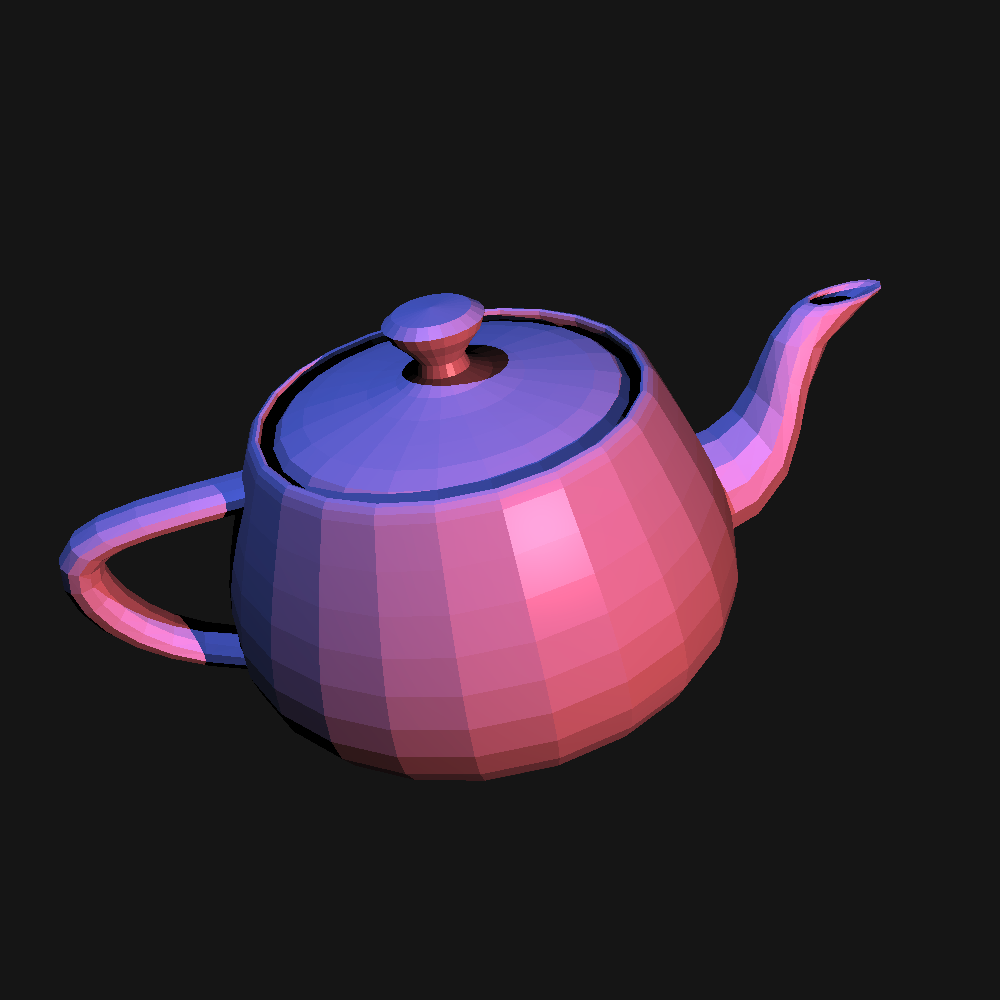
\includegraphics[width=5cm]{tekande}
  \caption{Rendering af en tekande.}
    \label{fig:tekande}
\end{figure}

Først køres programmet på den gamle algoritme:
\begin{lstlisting}
./trace teapot.old.ply
\end{lstlisting}
Terminaloutputtet er her illustreret i en listing:
\begin{lstlisting}
0.1%
0.2%
.
.
.
99.9%
100%
885s
\end{lstlisting}

Der ses altså at renderingstiden for figur \ref{fig:tekande} er på 885 sekunder med den gamle algoritme.

Programmet køres nu på det færdige program efter kd-træer er implementeret.
\begin{lstlisting}
./trace teapot.ply
\end{lstlisting}
Outputtet er:
\begin{lstlisting}
0.1%
0.2%
.
.
.
99.9%
100%
109s
\end{lstlisting}

Den nye renderings tid for figur \ref{fig:tekande} er på 109 sekunder efter optimeringen, det vil altså sige en forbedring på ca. 712\% og en faktisk stigning på 8.12 i forhold til den gamle algoritme. Der kan derfor udledes, at for figur \ref{fig:tekande} er det blevet over 8 gange så hurtigt at renderer figuren efter optimeringen. Krav 2 om optimering med KD-træer er derfor opfyldt.   